\exercice*

On considère le trinôme du second degré $f: x\mapsto (( a|facteur("X") )) (( b|facteur("so*x") )) (( c|facteur("so") ))$.

\begin{enumerate}
\item
\begin{enumerate}
    \item Soit $x\in\mathbb{R}$. Alors :
        \begin{align*}
            (( a|facteur )) \,\left( x (( -x1|facteur("so") )) \right) \, \left( x (( -x2|facteur("so") )) \right)
            &= (( a|facteur )) \,\left(x\times{} x (( -x1|facteur("so") ))\times{} x (( -x2|facteur("so") ))\times{} x (( -x1|facteur("so") ))\times{} (( -x2|facteur("p") )) \right) \\
            &= (( a|facteur )) \,\left(x^2 (( (-x1-x2)|facteur("so*x") )) (( (x1*x2)|facteur("so*") ))\right) \\
            &= (( a|facteur ))\times{} x^2 (( a|facteur("so") ))\times{} (( (-x1-x2)|facteur("p*x") )) (( a|facteur("so") ))\times{} (( (x1*x2)|facteur("p") )) \\
            &= (( a|facteur("X") )) (( b|facteur("so*x") )) (( c|facteur("so") ))\\
            &= f\,(x)
        \end{align*}
    \item Soit $x\in\mathbb{R}$. Alors :
        \begin{align*}
            (( a|facteur ))\,\left( x (( -alpha|facteur("so") )) \right)^2 (( beta|facteur("so") ))
            &= (( a|facteur ))\,\left( x^2 (( (-signealpha*2)|facteur("so") ))\times{} (( absalpha|facteur )) \times{} x + (( absalpha|facteur ))^2\right) (( beta|facteur("so") ))\\
            &= (( a|facteur ))\,\left( x^2 (( (-alpha*2)|facteur("so*x") )) + (( (absalpha**2)|facteur ))\right) (( beta|facteur("so") ))\\
            &=  (( a|facteur ))\times{} x^2 (( a|facteur("so") ))\times{} (( (-alpha*2)|facteur("p*x") )) (( a|facteur("so") ))\times{} (( (absalpha**2)|facteur )) (( beta|facteur("so") ))\\
            &= (( a|facteur("X") )) (( b|facteur("so*x") )) (( (a*absalpha**2)|facteur("so") )) (( beta|facteur("so") ))\\
            &= (( a|facteur("X") )) (( b|facteur("so*x") )) (( c|facteur("so") ))\\
            &= f\,(x)
        \end{align*}
\end{enumerate}
\item Résoudre les équations suivantes en choisissant la forme appropriée de $f$.
\begin{enumerate}
\item En prenant la forme factorisée, l'équation $f\,(x)=0$ est équivalente à l'équation produit nul $(( a|facteur ))\,(x (( -x1|facteur("so") )) )\,(x (( -x2|facteur("so") )) ) = 0$. Donc :
\begin{align*}
x (( -x1|facteur("so") ))=0 &\text{ ou } x (( -x2|facteur("so") ))=0 \\
x=(( x1|facteur )) &\text{ ou } x=(( x2|facteur ))
\end{align*}
Il y a donc deux solutions : $(( x1|facteur ))$ et $(( x2|facteur ))$.
\item $f\,(x)=(( c|facteur ))$ On remarque que la forme développée contient la constante $(( c|facteur ))$ : celles-ci devraient donc s'annuler, pour simplifier notre résolution.
\begin{align*}
f\,(x) &= (( c|facteur )) \\
(( a|facteur("X") )) (( b|facteur("so*x") )) (( c|facteur("so") )) &= (( c|facteur )) \\
(( a|facteur("X") )) (( b|facteur("so*x") )) (( c|facteur("so") )) (( -c|facteur("so") )) &= (( c|facteur )) (( -c|facteur("so") )) \\
(( a|facteur("X") )) (( b|facteur("so*x") )) &= 0 \\
\end{align*}
Nous pouvons maintenant factoriser le membre de gauche par $x$, ce qui nous donnera une équation produit nul.
\begin{align*}
(( a|facteur("X") )) (( b|facteur("so*x") )) &= 0 \\
(( a|facteur("x") ))\times{} x (( b|facteur("so") ))\times{} x &= 0 \\
x\,\left( (( a|facteur("x") )) (( b|facteur("so") )) \right) &= 0 \\
\end{align*}
\begin{align*}
x =0 &\text{ ou } (( a|facteur("x") )) (( b|facteur("so") ))=0 \\
x =0 &\text{ ou } (( a|facteur("x") )) =(( -b|facteur )) \\
x =0 &\text{ ou } x = \frac{(( -b|facteur ))}{(( a|facteur ))} \\
x =0 &\text{ ou } x = (( -(b/a)|facteur )) \\
\end{align*}
Il y a donc deux solutions : $x=0$ et $x=(( -(b/a)|facteur ))$.
\item $f\,(x)=(( beta|facteur ))$ On remarque que la forme canonique contient la constante $(( beta|facteur ))$ : en l'utilisant, elles devraient se simplifier.
\begin{align*}
f\,(x) &= (( beta|facteur)) \\
(( a|facteur )) \,\left( x (( -alpha|facteur("so") )) \right)^2 (( beta|facteur("so") )) &= (( beta|facteur ))\\
(( a|facteur )) \,\left( x (( -alpha|facteur("so") )) \right)^2 (( beta|facteur("so") )) (( -beta|facteur("so") )) &= (( beta|facteur )) (( -beta|facteur("so") ))\\
(( a|facteur )) \,\left( x (( -alpha|facteur("so") )) \right)^2 &= 0\\
\left( x (( -alpha|facteur("so") )) \right)^2 &= 0\\
\end{align*}
Or $0$ est le seul nombre dont le carré est nul, donc l'équation précédente est équivalente à :
\begin{align*}
x (( -alpha|facteur("so") )) &= 0\\
x &= (( alpha|facteur )) \\
\end{align*}
Il y a donc une unique solution $x=(( alpha|facteur ))$.
\end{enumerate}
\item
\begin{enumerate}
\item \emph{Dresser le tableau de variations de $f$.} Dans la forme développée, le coefficient devant le $x^2$ est 
(* if a > 0 *) positif (* else *) négatif (* endif *),
donc la fonction est 
(* if a > 0 *) décroissante puis croissante (* else *) croissante puis décroissante (* endif *).
De plus, l'absisse du sommet est $-\frac{(( b|facteur ))}{2\times{}(( a|facteur("p") ))}$, soit $(( alpha|facteur ))$, et
$f\,( (( alpha|facteur )) )=(( a|facteur ))\times{}(( alpha|facteur("p") ))^2 (( b|facteur("so") ))\times{} (( alpha|facteur("p") )) (( c|facteur("so") ))=(( beta|facteur ))$.
Le tableau de variations est donc :
\begin{center}
    \begin{tikzpicture}
      \tkzTabInit[espcl=2.5]
      {$x$/1, $f\,(x)$/1.5}
      {$-\infty$, $(( alpha|facteur ))$, $+\infty$}
      (* if a > 0 *)
      \tkzTabVar{+/, -/$(( beta|facteur ))$/, +/}
      (* else *)
      \tkzTabVar{-/, +/$(( beta|facteur ))$/, -/}
      (* endif *)
    \end{tikzpicture}
\end{center}
\item \emph{Dresser le tableau de signes de $f$.} Construisons un tableau de signes en utilisant la forme factorisée $f\,(x)=(( a|facteur )) \,\left(x (( -x1|facteur("so") ))\right) \, \left(x (( -x2|facteur("so") ))\right)$.

\begin{itemize}
\item Le premier facteur $x (( -x1|facteur("so") ))$ est une fonction affine, de coefficient directeur $a=1$ positif, et d'ordonnée à l'origine $b=(( -x1|facteur ))$. Elle est donc négative, puis positive, et change de signe en $-\frac{b}{a}=-\frac{(( -x1|facteur ))}{1}=(( x1|facteur ))$.
\item Le second facteur $x (( -x2|facteur("so") ))$ est aussi une fonction affine, de coefficient directeur $a=1$ positif, et d'ordonnée à l'origine $b=(( -x2|facteur ))$. Elle est donc négative, puis positive, et change de signe en $-\frac{b}{a}=-\frac{(( -x2|facteur ))}{1}=(( x2|facteur ))$.
\end{itemize}
\begin{center}
    \begin{tikzpicture}
      \tkzTabInit[lgt=4, espcl=2.5]
      {
        $x$/1,
        $(( a|facteur ))$/1,
        $x (( -x1|facteur("so") ))$/1,
        $x (( -x2|facteur("so") ))$/1,
        $f\,(x)=(( a|facteur ))\,\left( x (( -x1|facteur("so") )) \right)\,\left( x (( -x2|facteur("so") )) \right)$/1.5
      }
      {$-\infty$, $(( (x1, x2)|min|facteur ))$, $(( (x1, x2)|max|facteur ))$, $+\infty$}
      \tkzTabLine{, (( a|signe )), t, (( a|signe )), t, (( a|signe ))}
      (* if x1 < x2 *)
      \tkzTabLine{, -, z, +, t, +}
      \tkzTabLine{, -, t, -, z, +}
      (* else *)
      \tkzTabLine{, -, t, -, z, +}
      \tkzTabLine{, -, z, +, t, +}
      (* endif *)
      \tkzTabLine{, (( a|signe )), z, (( -a|signe )), z, (( a|signe ))}
    \end{tikzpicture}
\end{center}
\end{enumerate}
\item Répondre aux questions suivantes en utilisant le tableau de signes ou de variations.
\begin{enumerate}
\item \emph{Résoudre $f\,(x)\geqslant0$.} En regardant la dernière ligne du tableau de signes, on observe que $f$ est positive sur
(* if a > 0 *) les premier et dernier intervalles (* else *) l'intervalle central (* endif *).
Les solutions sont donc :
(* if a > 0 *)
   \[ x\in\interval[open left, scaled]{-\infty}{(( (x1, x2)|min|facteur ))} \cup \interval[open right, scaled]{(( (x1, x2)|max|facteur ))}{+\infty} \]
(* else *)
   \[ x\in\interval[scaled]{(( (x1, x2)|min|facteur ))}{(( (x1, x2)|max|facteur ))} \]
(* endif *)
\item \emph{Quel est l'extremum de $f$ ? Est-ce un maximum ou un minimum ? Pour quelle valeur de $x$ est-il atteint ?} On lit sur le tableau de variations que la plus
(* if a > 0 *) petite (* else *) grande (* endif *)
valeur prise par $f$ est $(( beta|facteur ))$. Le
(* if a > 0 *) minimum (* else *) maximum (* endif *)
de $f$ est donc $(( beta|facteur ))$, et il est atteint pour $x=(( alpha|facteur ))$.
\end{enumerate}
\end{enumerate}
